\documentclass{amsart}
\synctex=1

%=================================================================
% 
\newcount\DraftStatus  % 0 suppresses notes to selves in text
\DraftStatus=1   % TODO: set to 0 for final version
%=================================================================

%=================================================================
\usepackage{comment}
%=================================================================
%
\includecomment{JournalOnly}  
\includecomment{ConferenceOnly}  
\includecomment{TulipStyle}
%
%=================================================================
%=================================================================
% gitlatexdiff
%
%  https://gitlab.com/git-latexdiff/git-latexdiff
%=================================================================
%  git latexdiff HEAD  HEAD~5 --main templatex.tex
%  git latexdiff HEAD~1  --main templatex.tex
%  View pdf to see difference
%
%=================================================================
%
% Todo Notes for marginal comments
% 
%\newcount\DraftStatus  % 0 suppresses notes to selves in text
%\DraftStatus=1   % TODO: set to 0 for final version
\ifnum\DraftStatus=1
	\usepackage[draft,colorinlistoftodos,color=orange!30]{todonotes}
\else
	\usepackage[disable,colorinlistoftodos,color=blue!30]{todonotes}
\fi 
%\usepackage[disable]{todonotes} % notes not showed
%\usepackage[draft]{todonotes}   % notes showed
%
\makeatletter
 \providecommand\@dotsep{5}
 \def\listtodoname{List of Todos}
 \def\listoftodos{\@starttoc{tdo}\listtodoname}
 \makeatother
%
%=================================================================
%
\usepackage{amsmath}
\usepackage{amsfonts}
\usepackage{color}
\newcommand{\draftnote}[3]{ 
	\todo[author=#2,color=#1!30,size=\footnotesize]{\textsf{#3}}	}
% TODO: add yourself here:
%
\newcommand{\gangli}[1]{\draftnote{blue}{GLi:}{#1}}
\newcommand{\ShuxiaLin}[1]{\draftnote{red}{SXLin:}{#1}}
\newcommand{\WenbinJiang}[1]{\draftnote{green}{WBJiang:}{#1}}
\newcommand{\gliMarker}
	{\todo[author=GLi,size=\tiny,inline,color=blue!40]
	{Gang Li has worked up to here.}}
\newcommand{\SXLinMarker}
	{\todo[author=ShuxiaLin,size=\tiny,inline,color=red!40]
	{Shuxia Lin has worked up to here.}}
\newcommand{\WBJianginMarker}
	{\todo[author=WenbinJiang,size=\tiny,inline,color=green!40]
	{Wenbin Jiang has worked up to here.}}
%=================================================================

%=================================================================
%
% general packages
%  https://en.wikibooks.org/wiki/Category:Book:LaTeX
%  https://en.wikibooks.org/wiki/LaTeX/Package_Reference
%
%=================================================================
\usepackage{algorithm}
\usepackage{algorithmic}
\usepackage{subfiles}
\usepackage{indentfirst}
\usepackage{graphicx}
\usepackage{algorithm}
\usepackage{algorithmic}
\usepackage{breqn}
\usepackage{subcaption}
\usepackage{multirow}
\usepackage{psfrag}
\usepackage{url}
\usepackage{hyperref}
%\usepackage[colorlinks]{hyperref}
%\usepackage{cite}
\usepackage{cleveref}
\usepackage{booktabs}
\usepackage{rotating}
\usepackage{colortbl}
\usepackage{paralist}
%\usepackage{geometry}
\usepackage{epstopdf}
\usepackage{nag}
\usepackage{microtype}
\usepackage{siunitx}
\usepackage{nicefrac}
% for random text
\usepackage{lipsum}
\usepackage[english]{babel}
\usepackage[pangram]{blindtext}
% for tikz figures
\usepackage{tikz}
\usepackage{float}
\usetikzlibrary{fit,positioning,arrows.meta,shapes,arrows}
%\tikzset{neuron/.style={circle,thick,fill=black!25,minimum size=17pt,inner sep=0pt},
%	input neuron/.style={neuron, draw,thick, fill=gray!30},
%	hidden neuron/.style={neuron,fill=white,draw},
%	hoz/.style={rotate=-90}}
%
%=================================================================



\begin{TulipStyle}
\usepackage{natbib}
%=================================================================
%
% Version control information
%
%=================================================================
\usepackage{gitinfo2}
%=================================================================
\usepackage{fancyhdr}
\pagestyle{fancy}
\fancyhead{} % clear all header fields
\fancyhead[RO,LE]{\textsl{\rightmark}}
\fancyhead[LO,RE]{\ensuremath{\Rightarrow}
		\textbf{\textbf{[CONFIDENTIAL]}}\ensuremath{\Leftarrow}}
\fancyhead[CO,CE]{}
%=================================================================
\fancyfoot{} % clear all footer fields
\fancyfoot[CE,CO]{\textbf{\thepage}} 
\fancyfoot[LO,LE]{
\includegraphics[height=.9\headheight]{logos/tulip-logo.eps}
		\gitVtagn-\gitBranch\ (\gitCommitterDate)}
\fancyfoot[RO,RE]{Committed by: \textsl{\gitCommitterName}}

\setlength{\headheight}{12pt}
\renewcommand{\headrulewidth}{0.4pt}
\renewcommand{\footrulewidth}{0.4pt}
%=================================================================


%=================================================================
% for math notations
% ----------------------------------------------------------------
\usepackage{mathtools}
\usepackage{amsthm}
%
% THEOREMS -------------------------------------------------------
%
\newtheorem{thm}{Theorem}[section]
\newtheorem{cor}[thm]{Corollary}
\newtheorem{lem}[thm]{Lemma}
\newtheorem{prop}[thm]{Proposition}
\theoremstyle{definition}
\newtheorem{defn}[thm]{Definition}
\theoremstyle{remark}
\newtheorem{rem}[thm]{Remark}
\numberwithin{equation}{section}
% MATH -----------------------------------------------------------
\newcommand{\norm}[1]{\left\Vert#1\right\Vert}
\newcommand{\abs}[1]{\left\vert#1\right\vert}
\newcommand{\set}[1]{\left\{#1\right\}}
\newcommand{\Real}{\mathbb R}
\newcommand{\eps}{\varepsilon}
\newcommand{\To}{\longrightarrow}
\newcommand{\BX}{\mathbf{B}(X)}
% ----------------------------------------------------------------
\newcommand{\I}{{\cal I}}
\newcommand{\Id}{{\cal I} }
\newcommand{\Dc}{{\cal D}}
\newcommand{\J}{{\cal J}}
\newcommand{\Dn}{{\cal D}_n}
\newcommand{\Dd}{{\cal D}_n }
\renewcommand{\P}{{\cal P}}
\newcommand{\Nu}{{\cal N} }
\newcommand{\B}{{\cal B}}
\newcommand{\Bf}{{\bf B}}
\newcommand{\Y}{{\bf Y}}
\newcommand{\A}{{\cal A}}
% ----------------------------------------------------------------
\newcommand{\V}{{\cal V}}
\newcommand{\M}{{\cal M}}
\newcommand{\F}{{\cal F}}
\newcommand{\Fd}{{\cal F}}
\newcommand{\BF}{{\cal BF}_n}
\newcommand{\BFd}{{\cal BF}_n}
\newcommand{\TF}{{\cal TF}_n}
\newcommand{\TFd}{{\cal TF}_n}
%\newcommand{\G}{{\cal G}}
\newcommand{\X}{{\cal X}}
\newcommand{\E}{{\cal E}}
\newcommand{\K}{{\cal K}}
\newcommand{\T}{{\cal T}_n}
\renewcommand{\H}{{\cal H}}
% ----------------------------------------------------------------
\newtheorem{Remark}{Remark}
\newtheorem{proposition}{Proposition}
\newtheorem{theorem}{Theorem}
\newtheorem{lemma}{Lemma}
\newtheorem{corollary}{Corollary}
\newtheorem{example}{Example}
\newtheorem{definition}{Definition}
\newtheorem{Algorithms}{Algorithm}
% ----------------------------------------------------------------
\newcommand{\bu}{{\mathbf 1} }
\newcommand{\bo}{{\mathbf 0} }
\newcommand{\N}{\mbox{{\sl l}}\!\mbox{{\sl N}}}
% ----------------------------------------------------------------
\def\uint{[0,1]}
\def\proof{{\scshape Proof}. \ignorespaces}
\def\endproof{{\hfill \vbox{\hrule\hbox{%
   \vrule height1.3ex\hskip1.0ex\vrule}\hrule
  }}\par}
%
%=================================================================

\hypersetup
{
    pdfauthor={\gitAuthorName},
    pdfsubject={TULIP Lab},
    pdftitle={},
    pdfkeywords={TULIP Lab, Data Science},
%	bookmarks=true,  
}

\end{TulipStyle}




%=================================================================
%
\begin{document}
%
%=================================================================
%
\title[Chen Jin's Flip00 ]{Flip00 Final Presetantion Report}%

\author{Jin Chen}
\address[A.~1]{,\\ Business school of HuNan University, Changsha , China}%


%\author{Gang Li}
%\address[A.~2]{School of Information Technology \\
%Deakin University, Geelong, VIC 3216, Australia}%
%\email[A.~2]{gang.li@deakin.edu.au}


%\author{Author 3}
%\address[A.~3]{School of Information Technology \\
%Deakin University \\
%Vic 3125, Australia}%
%\email[A.~3]{xxx@deakin.edu.au}

%\thanks{Thanks to \ldots}%
%\subjclass{Artificial Intelligence}%
\keywords{Machine Learning, Data Mining, ...}%
\date{\gitAuthorDate}%

\begin{abstract}
This report contains four parts. 
first, 
introduce the problem and describe the data. 
Second, 
visualize the data to find some potential relationships 
between the attribute values.
Afterwards,process the data 
like creating the dummy variables, feature engineering, feature selection etc. 
Third, 
explain the method of experiment.Then, experiment and 
analyze the performance of different models.
The last part is conclusion . 
\end{abstract}

\maketitle
\tableofcontents

\newpage
%=================================================================

%=================================================================

\section{Introduction}\label{sec-intro}

\subsection{Problem Statement}
\

The data contains the location and circumstances of every field goal 
attempted by Kobe Bryant took during his 20-year career. The task is to predict 
whether the basket went in (shot_made_flag).




\subsection{Data List}
\

For example,the action_type,shot_made_flag,  
shot_type and shot_zone_area are part of the attributes of each sample,
the fllowings are the meaning of some attributes.

\begin{table}[htbp]
	\centering
	\begin{tabular}{cc}
		\toprule  %????????
		Attribute& Note\\
		\hline
		action_type & Jumpshot,Layup,Dunk,Tipshot,Hookshot,Bankshot\\
		loc_x ,loc_y & shots point\\
		shot_made_flag & 1=Yes,0=No\\
		shot_type & 2PT Field Goal,3PT Field Goal\\
		shot_zone_area & shots area by area\\
		shot_zone_basic & shots area by  NBA rules\\
		shot_zone_range & shots area by radius\\
		
		\bottomrule %????????
	\end{tabular}
	\bigskip
	\caption{Data Information}
\end{table}
\label{table1}



\subsection{Problem Analysis}

\subsubsection{Train Data and Test Data}
\
There are 30697 lines of data in the training set.I will split the dataset as training sets and testing sets.
They have removed 5000 of the shot_made_flags (represented as missing values in the csv file). 2cfd the test set shots for which we need submit a prediction. We are provided
a sample submission file with the correct shot_ids needed for a valid prediction.


\subsubsection{Problem Possible Solutions}
\
After analyse the dataset by some simple visualizations.
In the process of date preparation,I will engineer the feature to improve the model accuracy,
then,create some dummy variables.
There are many machine learning moodel
can solve the two classification problem,
such as The RandomForestClassifier,
KNeighbors Classifier and Logistic Regression.
Finaly,make a final prediction,fit the model with whole data





\section{Exploratory Data Analysis} \label{sec-data_exploration}

\subsection{Data Information}
\

The following  ~\cref{tbl:data information}
is the statistical result of the columns.
From this table,we can discover that some of columns have a similar meaning 
or may not contribute much to the model.
so we may need remove and convert them. 
\newpage

\begin{table}[htbp]  \centering
	\caption{Data Information}
	\label{tbl:data information}		
	\begin{tabular}{ccccccc}
		\hline
		% after \\: \hline or \cline{col1-col2} \cline{col3-col4} ...
		 & loc\_x & loc\_y & lon & min\_remaining & sec\_remaining \\
		\hline
		count & 30697 & 30697 & 30697 & 30697 & 30697  \\
		mean  & 7.110499	& 91.107535 & -118.262690 & 4.885624 & 28.365085\\
		std 	& 110.124578 & 87.791361 & 0.110125	& 3.449897 & 17.478949  \\
		min 	& -250.000000 & -44.000000 & -118.519800 & 0.000000	& 0.000000  \\
		25\%  & -68.000000 & 4.000000 & -118.337800 & 2.000000 & 13.000000\\
		50\%  & 0.000000	& 74.000000	& -118.269800	& 5.000000	& 28.000000	\\
		75\% & 95.000000 & 160.000000 & -118.174800 & 8.000000 & 43.000000 \\
		max  & 248.000000 & 791.000000 & -118.021800 & 11.000000 & 59.000000 \\
		\hline 
		%\bottomrule
	\end{tabular}
\end{table}

\subsection{Data Visualization}
\

Use EDA to plot the distribution of the data,
can observate the data intuitively and
find the relation between the attribute values. 
For example histogram can visually observe 
the distribution of numerical variables, 
scatterplot can show their distribution trends 
and whether exists outliers.
For classification problems, 
the data with the same label is drawn in same color, 
which is very helpful for 
the construction of the Feature.

\subsubsection{ Histogram}
\

The figure 1
shows the hit distribution of Kobe's shots  
the figure 2
is the visualization of two kinds of shots(two-point shot and three-point shot).
It can be seen that the number of shots and hit rate of the 2PT ball are extremly high. 
While the percentage of 3PT shots is relatively low.
the figure 3 
shows the shot accuracy of various action type.
It can be seen that dunk is the highest hit rate, followed by bank shot is about 80\%,
while jump shot and Tip shot are relatively difficult.

\begin{figure}[H]

		\centering
		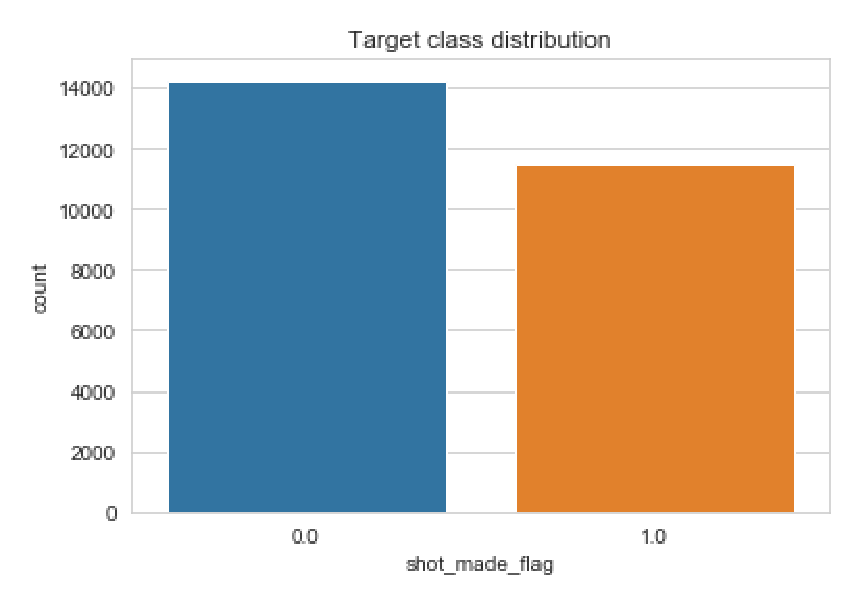
\includegraphics[scale=0.6]{c.eps}
		\caption{target class distribution}
	

		\centering
		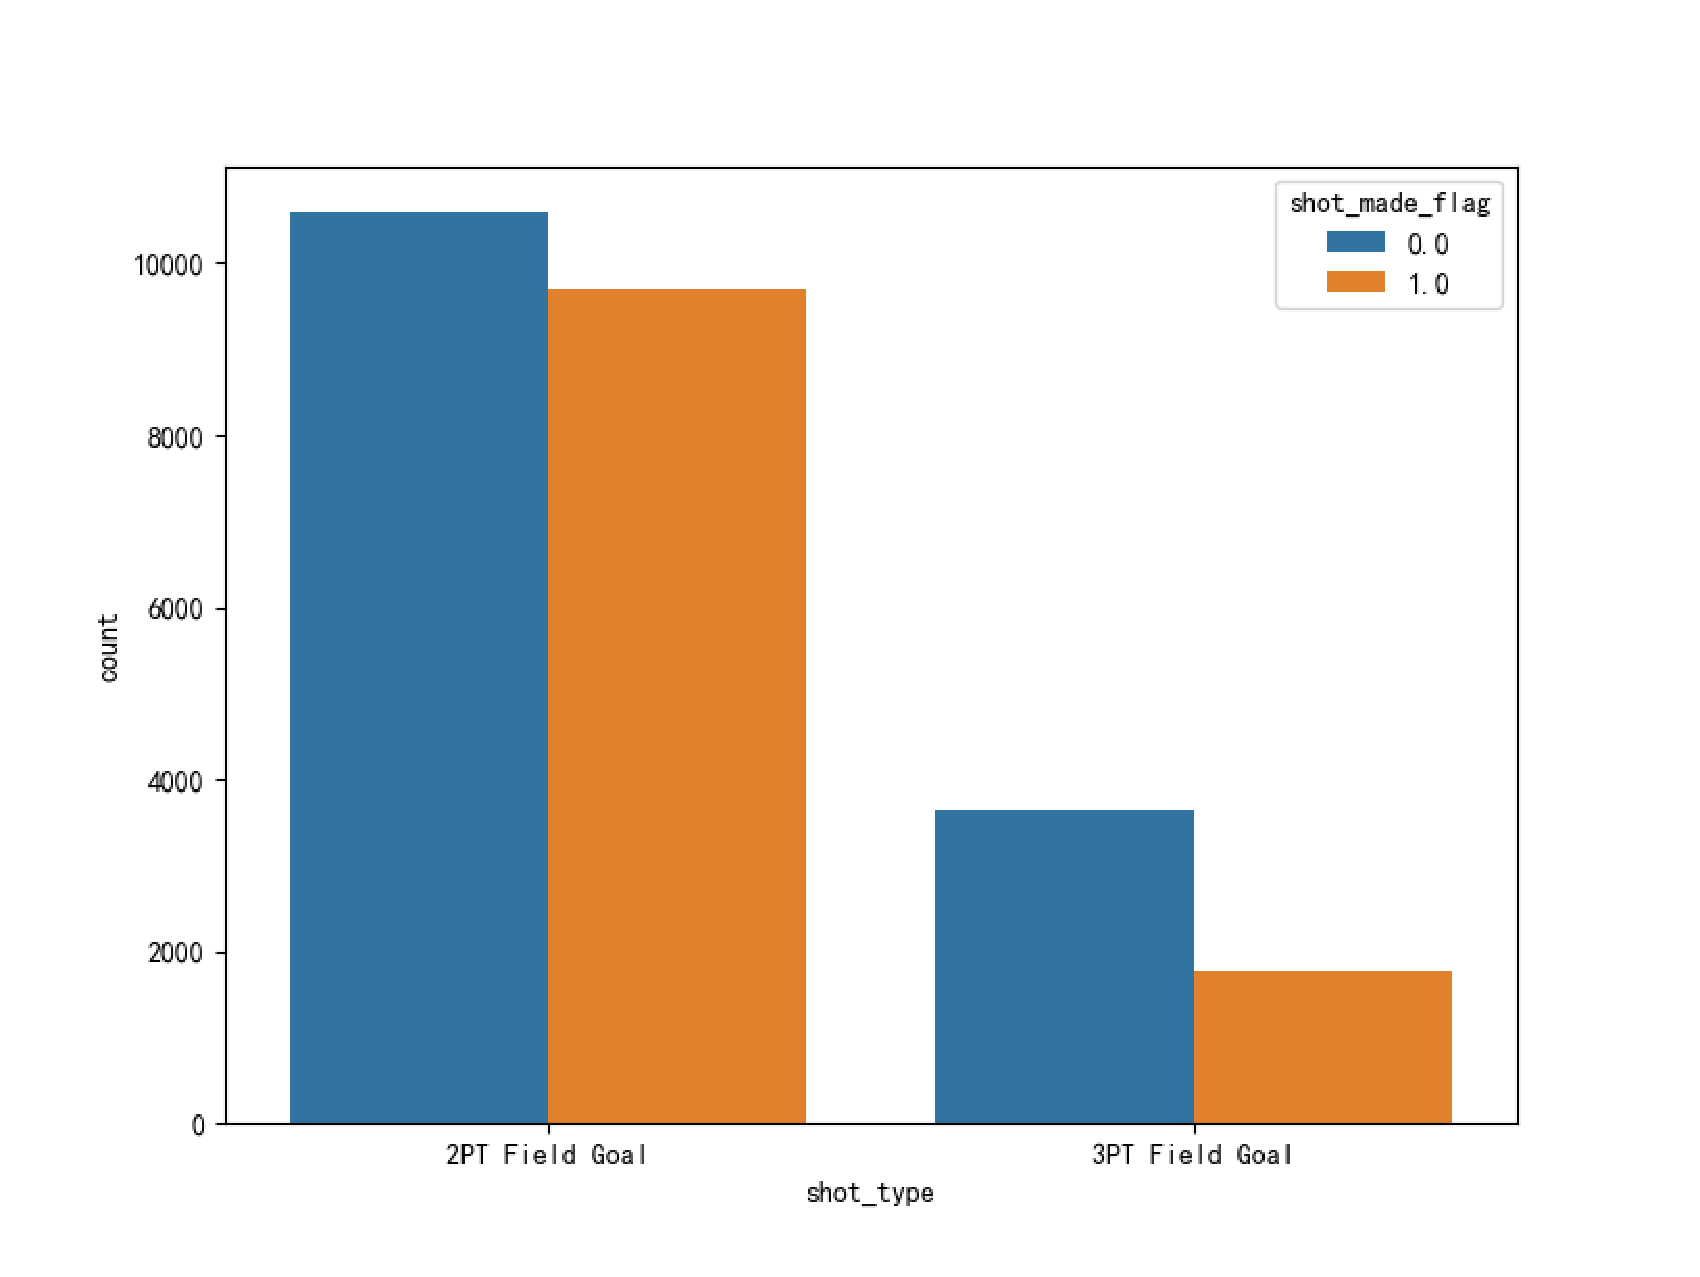
\includegraphics[scale=0.4]{d.eps}
		\caption{The hit distribution histogram of two shot types}
		
			\centering
		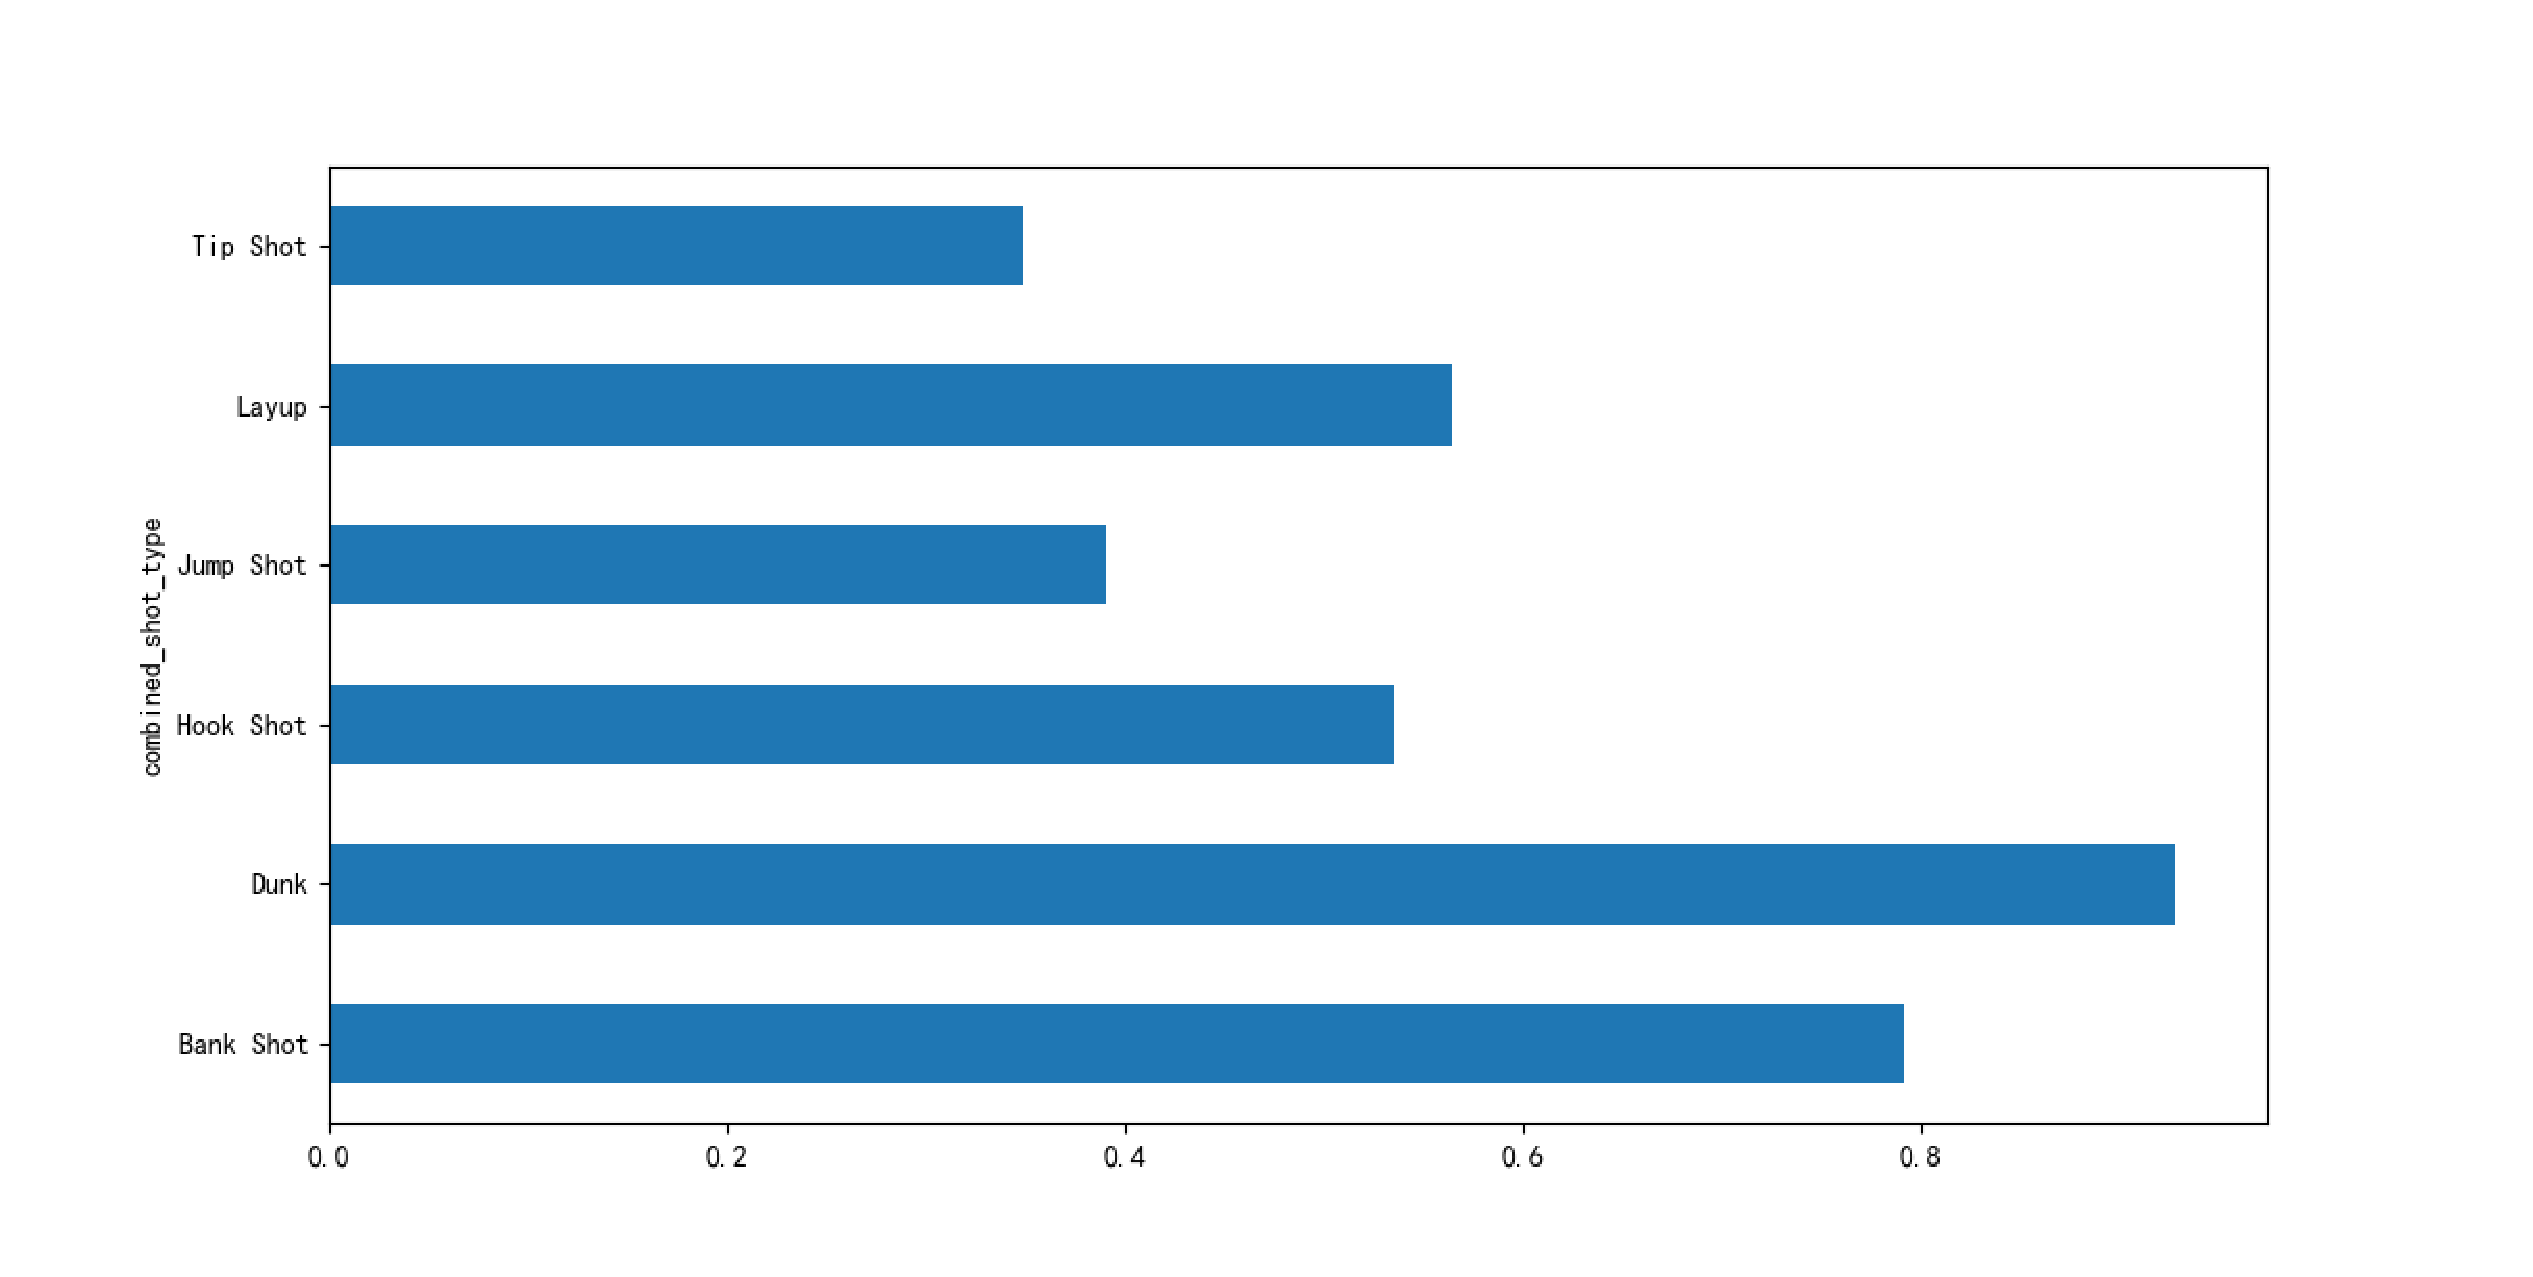
\includegraphics[scale=0.3]{f.eps
		}        %Õâ¸öÊÇÔÚLaTeXÎļþ¼ÐÖеÄÏà¶Ô·¾¶
		\caption{the shot accuracy of various action type}
		\label{fig3}
	
\end{figure}


\subsubsection{Scatter Plot}
\

Using the scatter plot we can combine multiple 
categorical value series on to the same chart distinguishing them using color or 
variation in symbol.
Lets get some understanding about the different zones and the shots made from zones.
\begin{figure}[H]
		\centering
	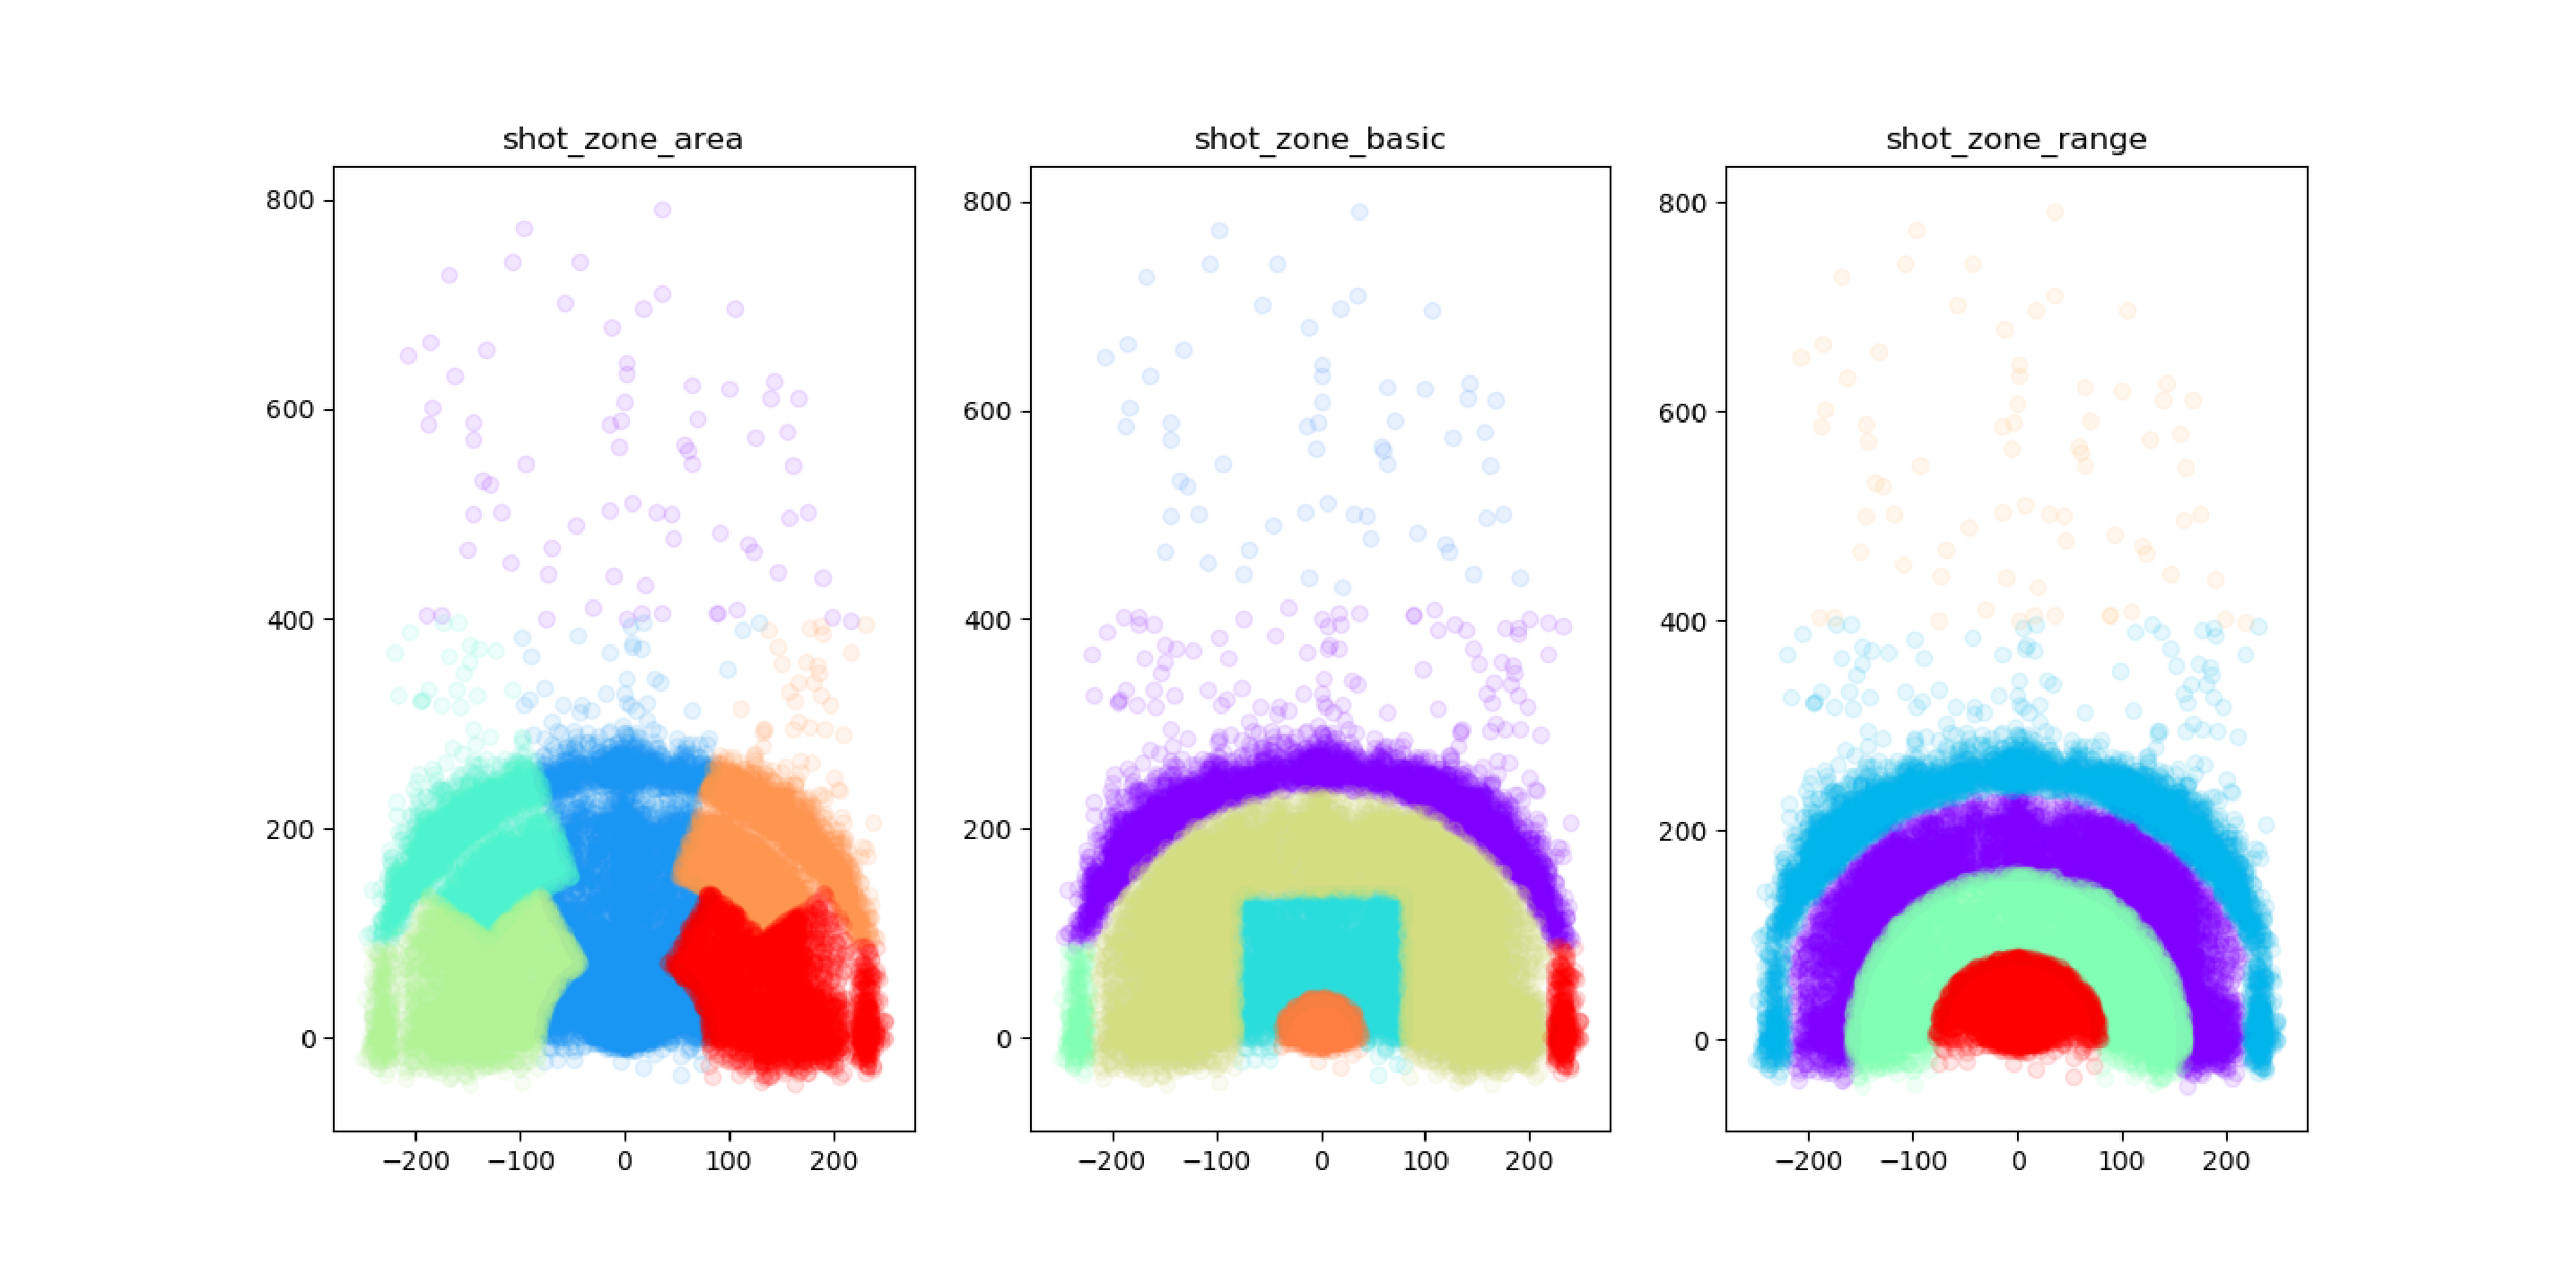
\includegraphics[scale=0.3]{h.eps
	}        %Õâ¸öÊÇÔÚLaTeXÎļþ¼ÐÖеÄÏà¶Ô·¾¶
	\caption{Division of shooting area}
	\label{fig4}

\end{figure}

\subsubsection{Line Chart}
\

The line chart can not only show the quantity, but also clearly see the increase and decrease of data.
Lets now see the Kobe's shots positioning with the time and distance.

\begin{figure}[H]
	\centering
	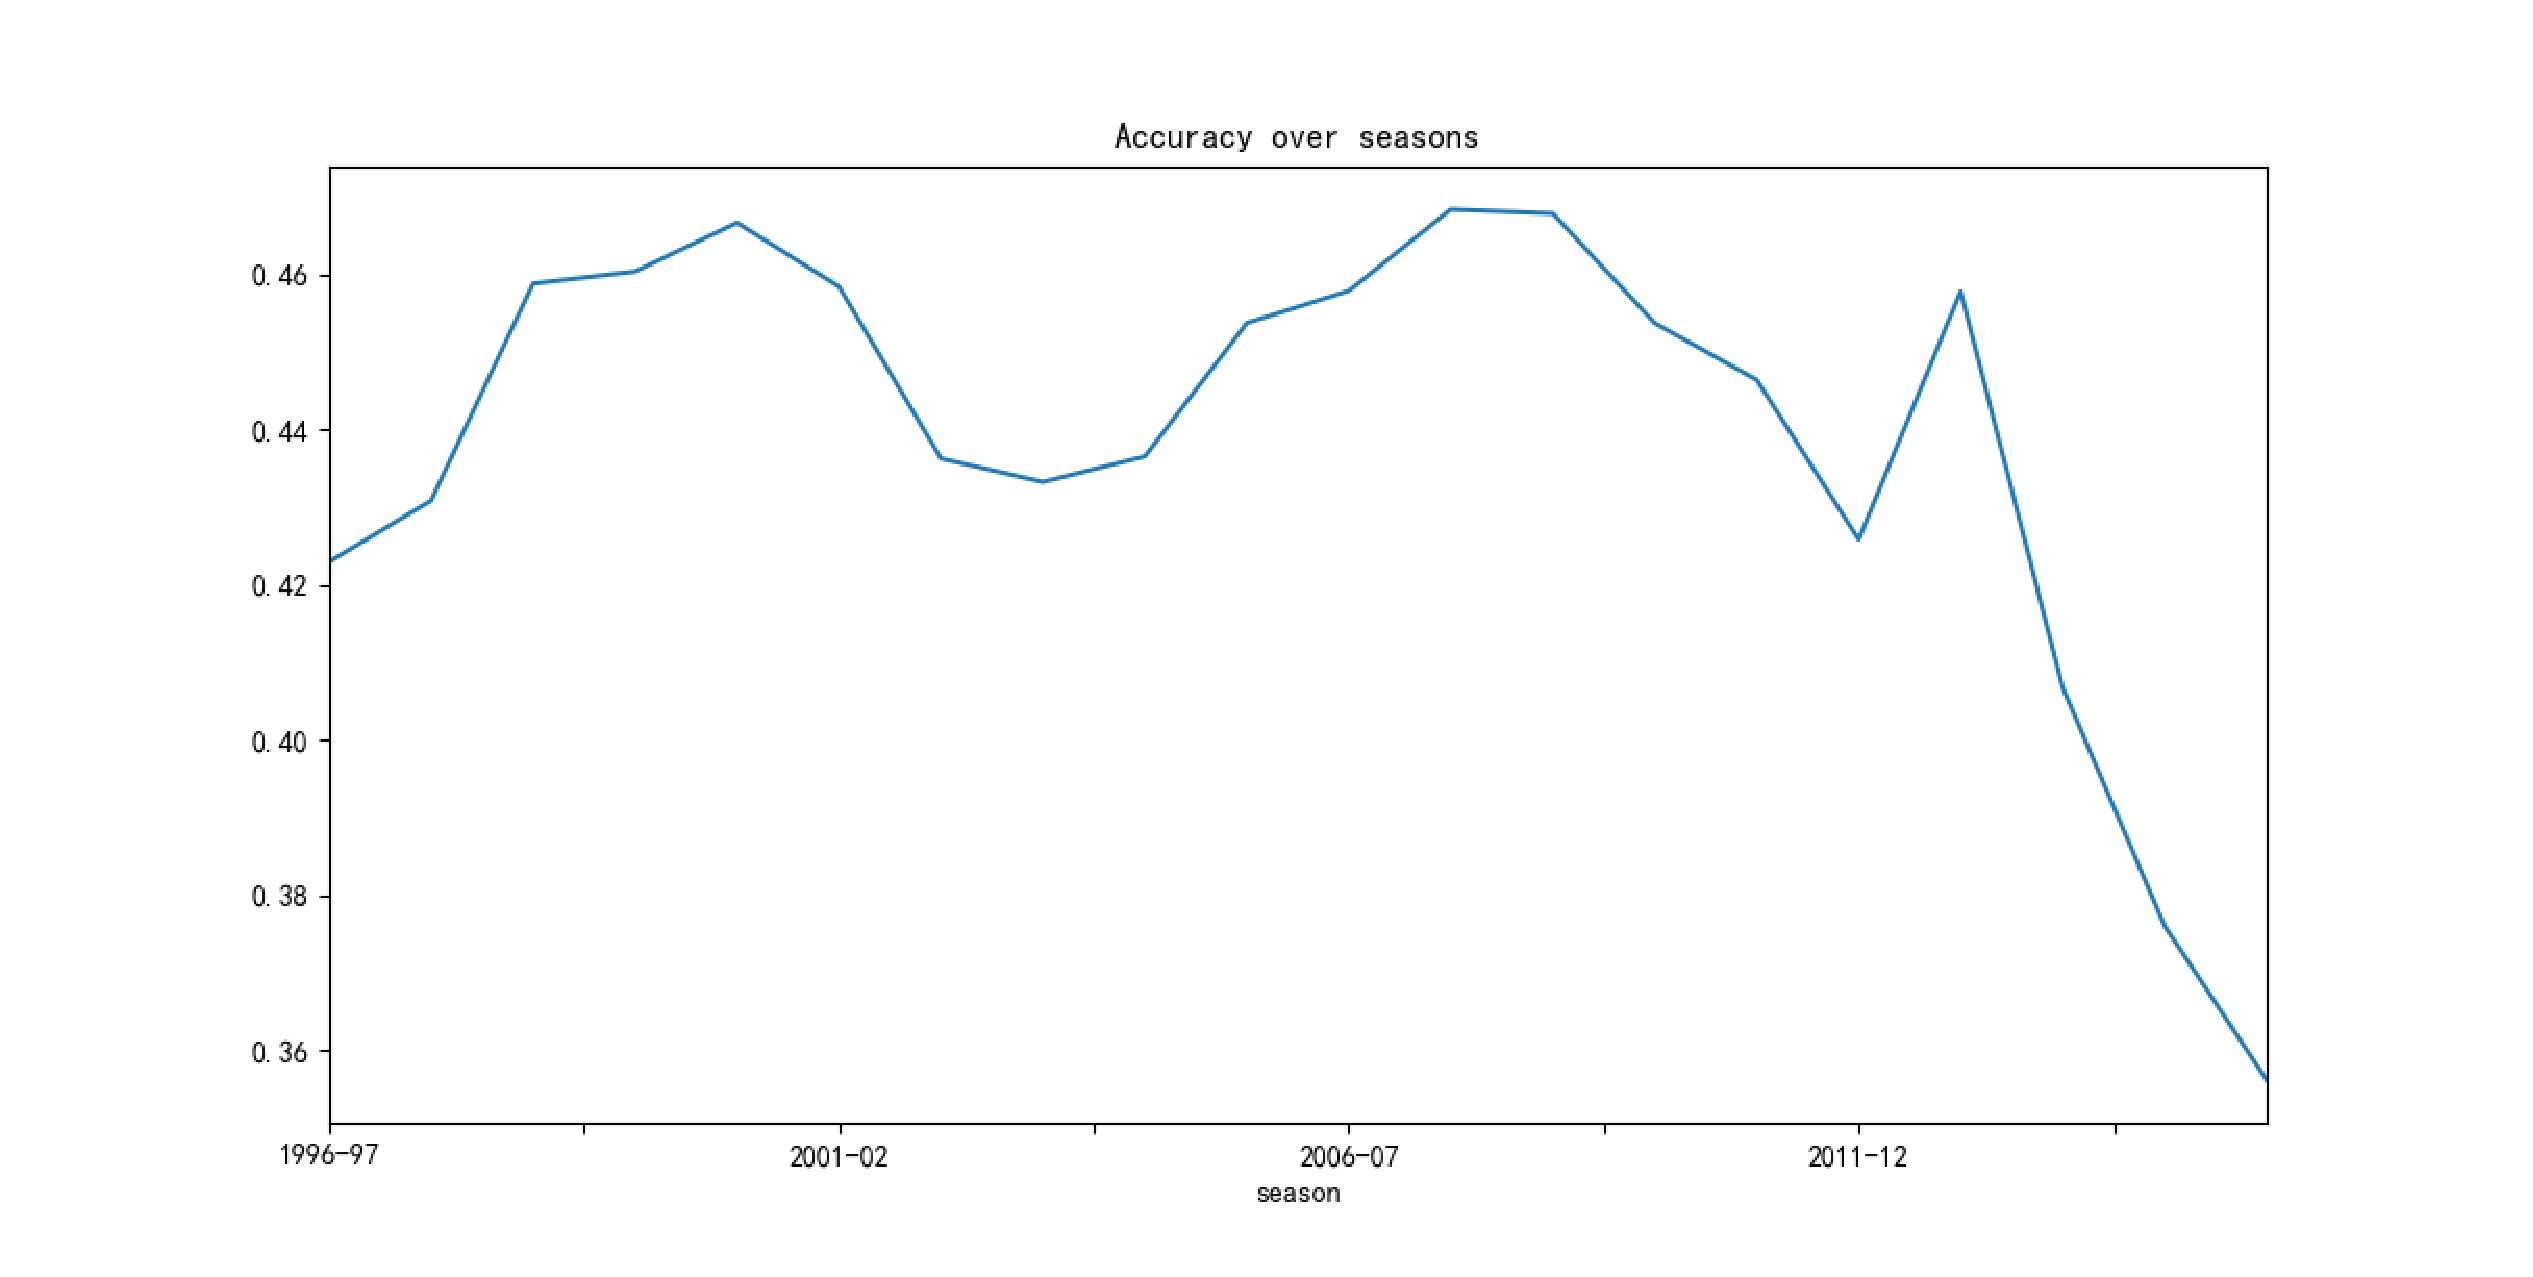
\includegraphics[scale=0.28]{m.eps
	}        %Õâ¸öÊÇÔÚLaTeXÎļþ¼ÐÖеÄÏà¶Ô·¾¶
	\caption{shot accuracy of each seasons}
	\label{fig5}
\end{figure}

\begin{figure}[H]
	\centering
	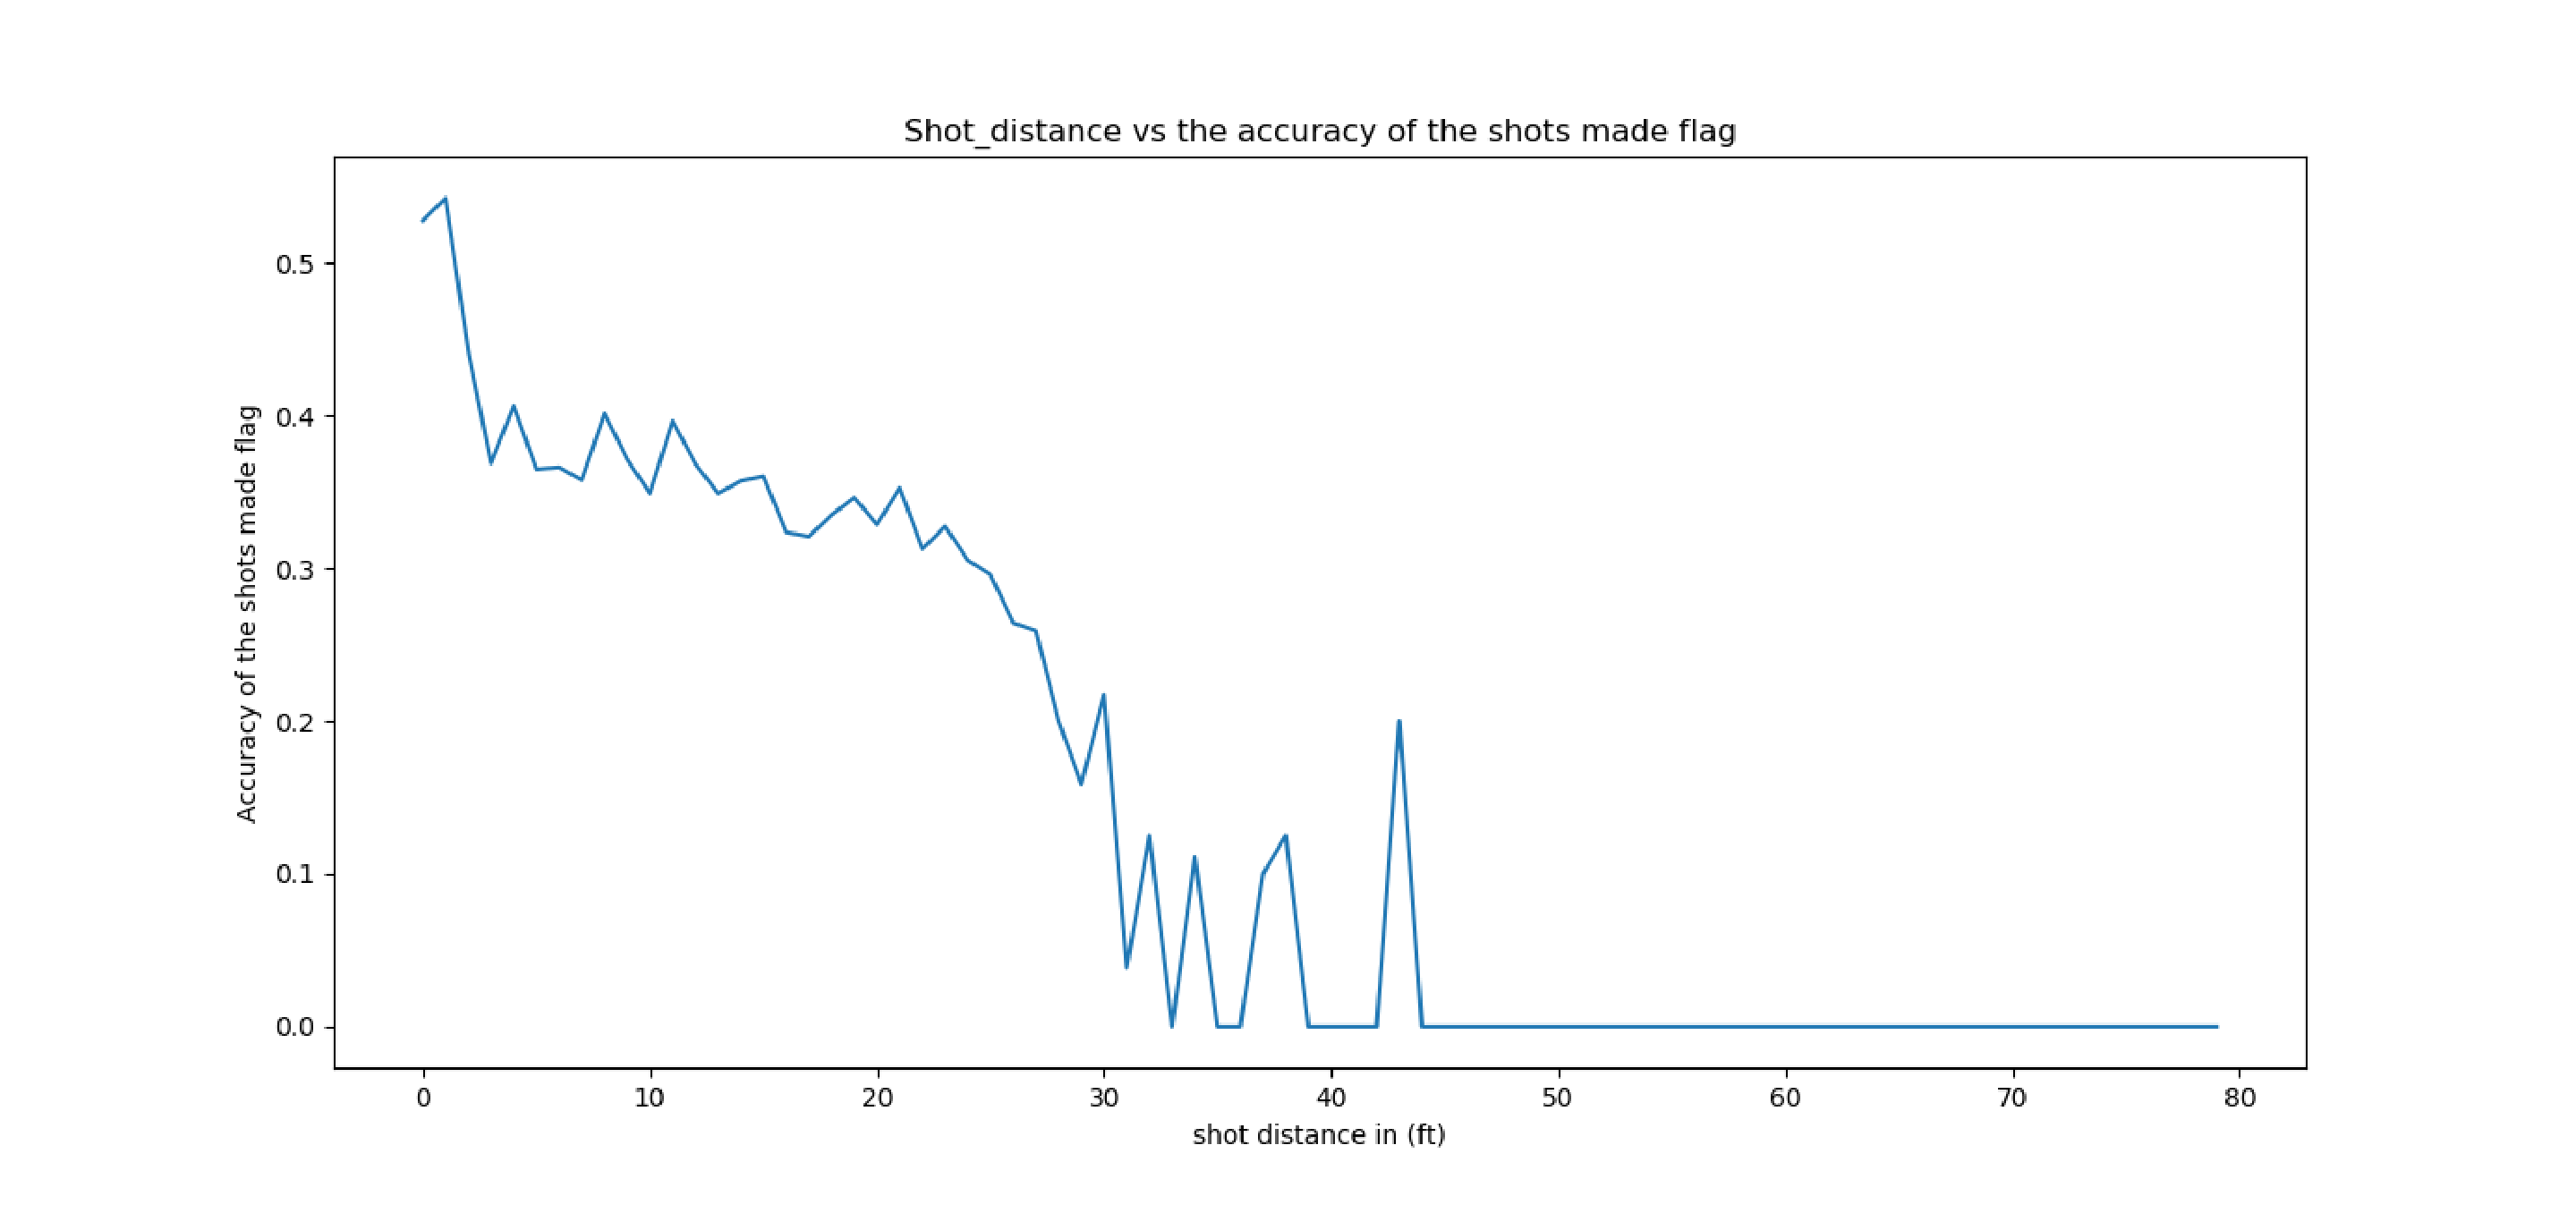
\includegraphics[scale=0.28]{s.eps
	}        %Õâ¸öÊÇÔÚLaTeXÎļþ¼ÐÖеÄÏà¶Ô·¾¶
	\caption{Shot_distance vs the accuracy of the shots made flag}
	\label{fig6}
\end{figure}
\newpage
\subsection{Data Preparation}

\subsubsection{Data Cleaning}
\

As it can be seen from 
the picture that, (loc_x ,loc_y) and (lat , lon) represent the same.
So, drop one of those.
Meanwhile,some attributes have no attribution for our model,
Therefore some columns might be dropped.
similarly,there is no real use of the columns team_id, team_name, game_event_id, game_id.
So, removing them is a good option.The opponent and the matchup also represents the same thing, 
so remove the matchup column.The game_date and shot_id also has no use.
Since, we have equal attacks from both sides we can remove the shot_zone_ares as it
doesnt contribute much to the model, we can also remove the shot_zone_basic for the same reason.


\begin{figure}[H]
	\centering
	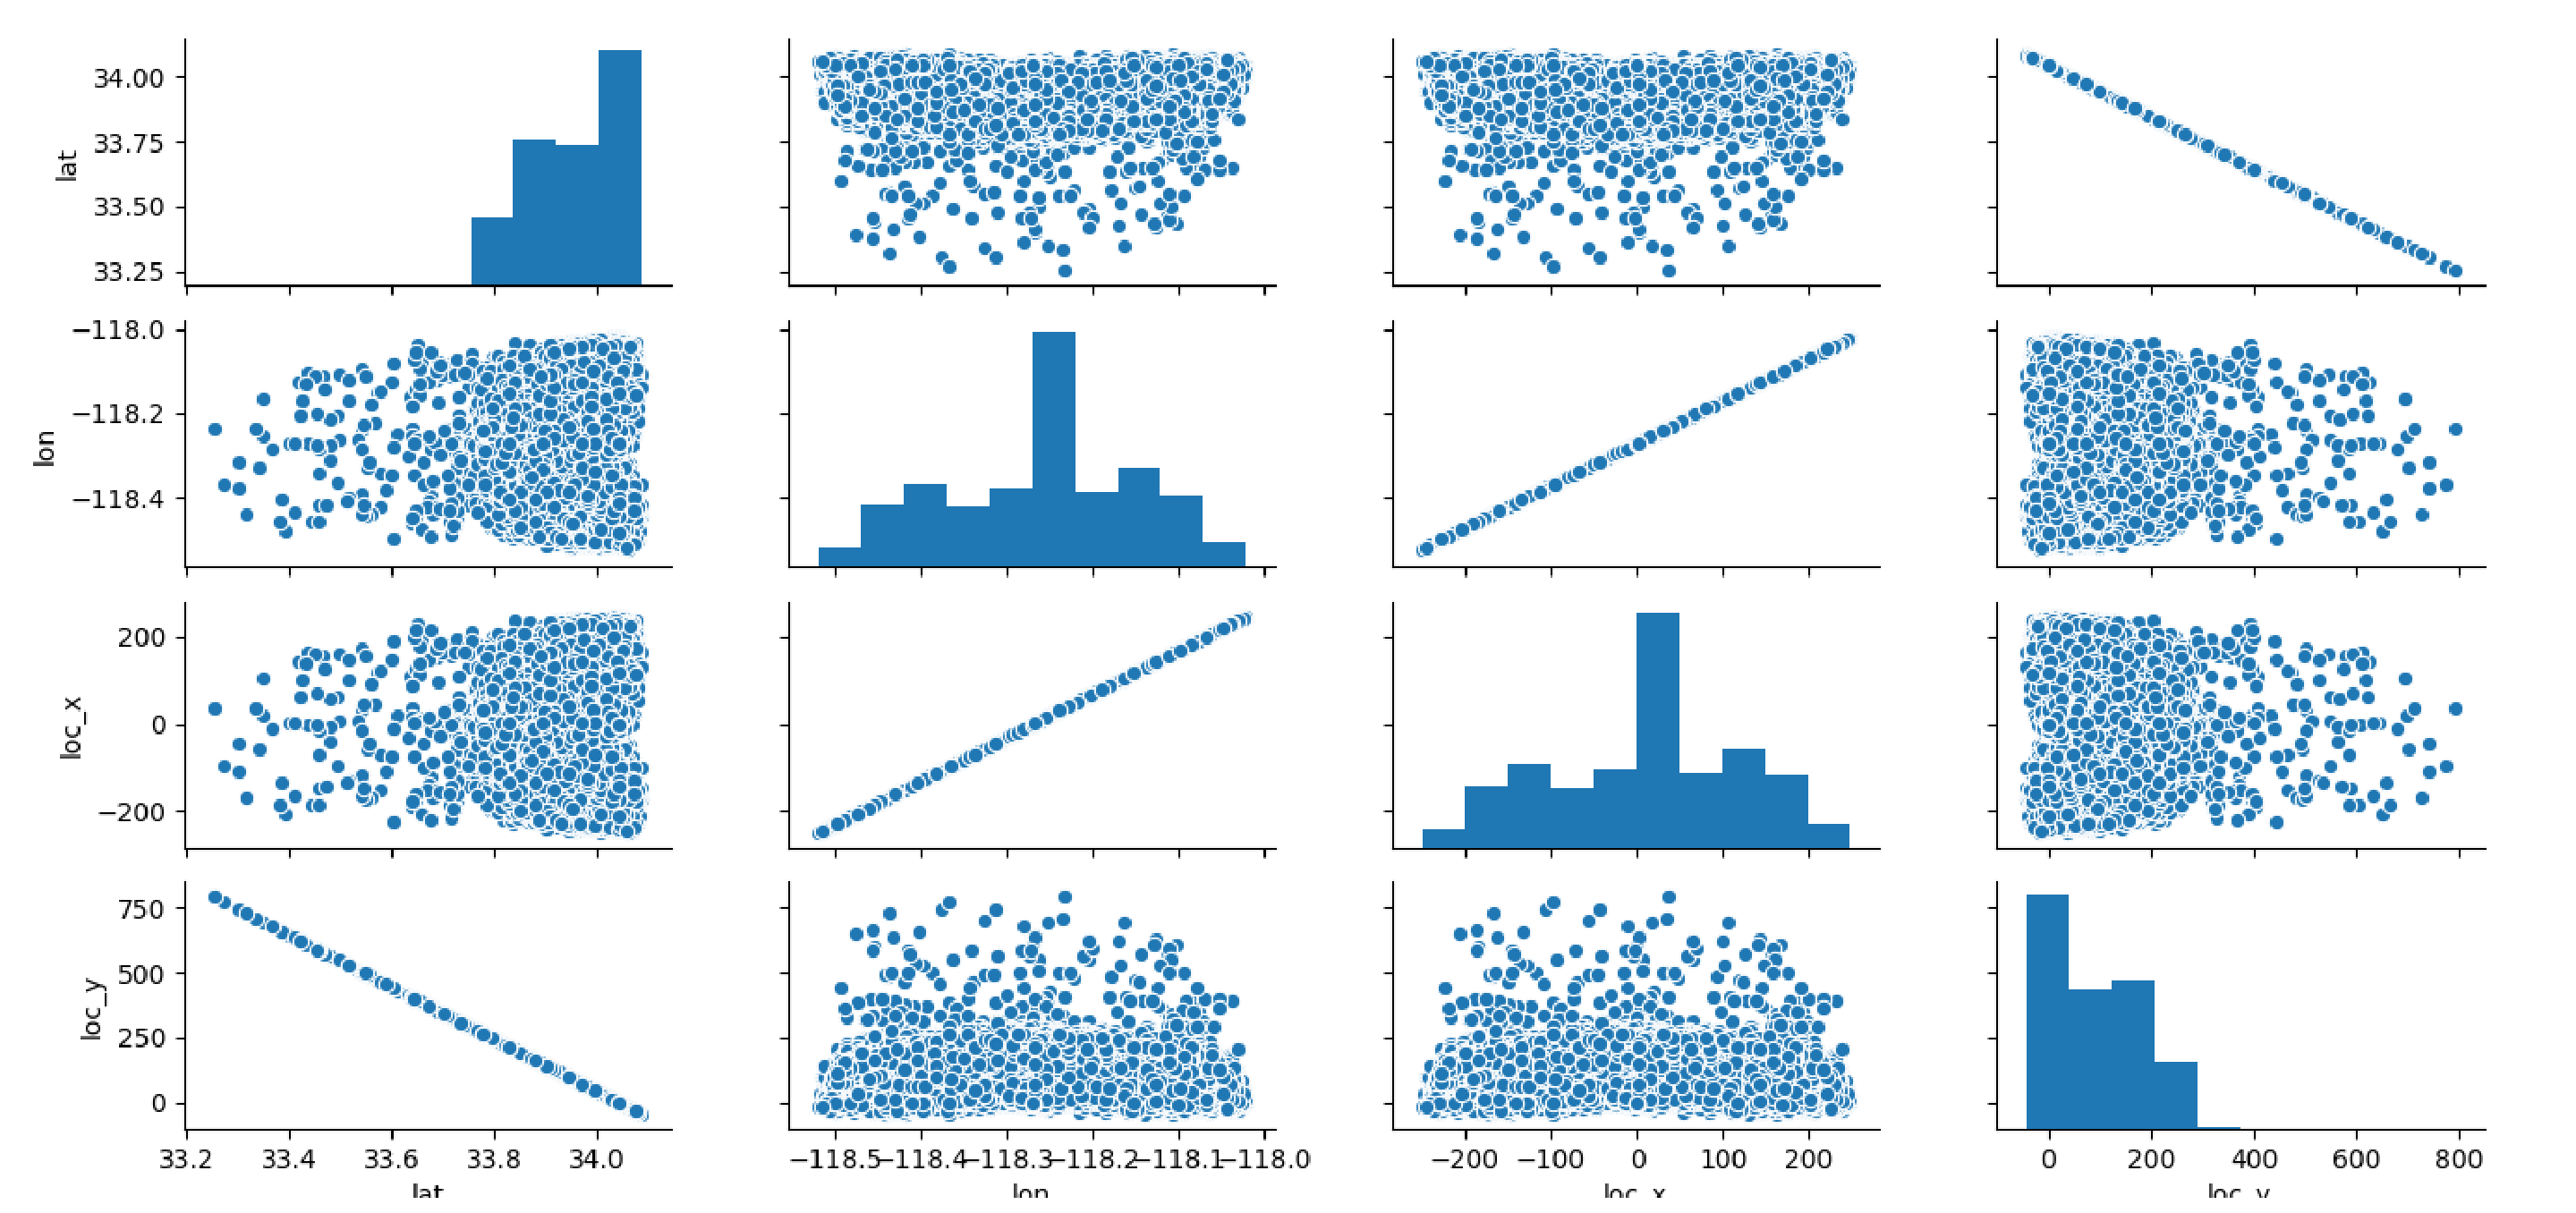
\includegraphics[scale=0.25]{t.eps
	}        %Õâ¸öÊÇÔÚLaTeXÎļþ¼ÐÖеÄÏà¶Ô·¾¶
	\caption{Pairplot of (loc\_x ,loc\_y) and (lat , lon)}
	\label{fig7}
\end{figure}


\subsubsection{Data Transformation}
\

After deleted all the useless columns,we need to merge some features,and create the dummy variables.
First,Let's convert the minutes and seconds to single column.
\begin{description}
	\item[total\_seconds] row[seconds\_remaining]*row[minutes\_remaining] 
\end{description}
After that,we can remove the minutes and the seconds columns.
Categorical variables such as action_type,combined_shot_type,season,shot_type,shot_zone_range 
and opponent,we can create the dummy variables for further analysis.
\begin{figure}[htbp]
	\centering
	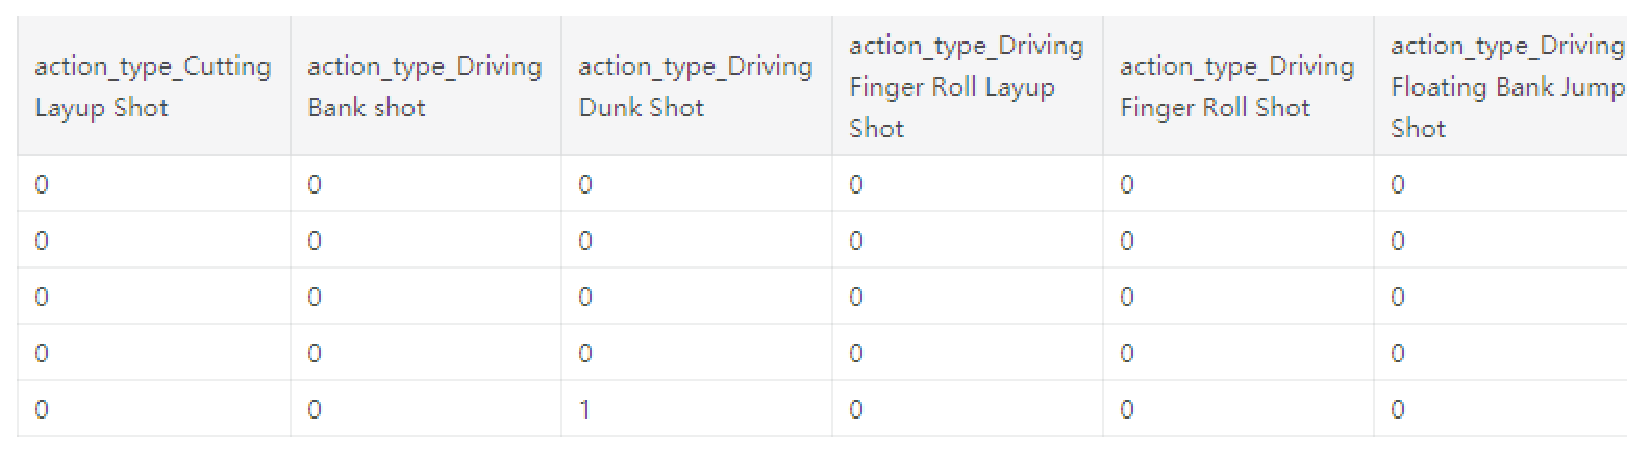
\includegraphics[scale=0.3]{u.eps
	}        %Õâ¸öÊÇÔÚLaTeXÎļþ¼ÐÖеÄÏà¶Ô·¾¶
	\caption{part of the converted dataset}
	\label{fig8}
\end{figure}

\section{Methods}

There are many machine learning algorithms 
for classification problem. 
Choose the following algorithms
as the base models of ensemble model,show the most important parameters.

\begin{itemize}
	\item RandomForest 
	%\item Bagging
	%\item GradientBoosting
	\item LogisticRegression

	\item KNeighbors 

\end{itemize}
\subsection{Models}
\

The base models have many parameters,
select the some parameters that 
have a larger impact on 
the forecast results,
the use Grid Search to find 
the optimal paratemers set.	
The following is training result. 
\subsubsection{RandomForest}
\

Random forest is a classifier with 
multiple decision trees, and
the output is determined by 
the mode of the individual tree output.


\begin{description}
	\item[n_estimators] the number of decision trees
	\item[criteriom] criterion of choosing 
	the most appropriate node
	\item[max_depth] The maximum depth of the tree, 
	the default is None 
	\item[max_features] The feature that is divided 
	when selecting the optimal attribute 
	cannot exceed this value.
\end{description}




\subsubsection{LogisticRegression}
\

Logistic regression is the algorithm that 
processing a large amount of 
observation data to 
obtain mathematical expressions 
that are in line with 
the internal laws of things


\begin{description}
	\item[Penalty] Regular function
	\item[C] Regular coefficient
\end{description}

%J=sum(logloss(f(xi), yi)) + C* penalty


%\frac{\partial f}{\partial x} = 2\,\sqrt{a}\,x

\subsubsection{KNeighbors}
\

The meaning of the knn algorithm is that 
enter new data without tags, 
compare each feature of the new data with 
each feature in the training set, 
and select the classification tag with 
the most similar feature (nearest neighbor: k)


\begin{description}
	\item[n_neighbors] number of neighbors to use 
	by default for kneighbors queries
	\item[leaf_size] leaf size passed to BallTree or KDTree
	\item[p] power parameter for choosing 
	the distance calculation formula
	\item[weights] used in prediction
	\item[algorithm] compute the nearest neighbors
\end{description}

	
\subsection{Forcast Result}

\

The following are the best parameters and 
the Best Score in training of 
the base models 
in original train data. 

\begin{itemize}
	\item Best Parameters of Models
	\begin{description}
		\item[RandomForest] 'criterion': 'entropy', 'max\_depth': 5, 
		'max\_features': None, 'n\_estimators': 100
		\item[LogisticRegression] 'C': 1, 'penalty': '11'
	
		\item[KNeighbors] 'algorithm': 'auto', 'leaf\_size': 10, 
		'n\_neighbors': 20, 'p': 5, 'weights': 'uniform'

	\end{description}
	
	
\item Model Accuracy 
\newline
From the  ~\Cref{tbl:best_score_base_models_old},
it shows that the accuracy of 
each model is not much different.
and  it has shown that logistic regression runs better than others.
	\begin{table}[h]  
		\centering
		\caption{Accuracy of these Models}
		\label{tbl:best_score_base_models_old}
		\begin{tabular}{cccc}
			%\bottomrule
			\toprule
			& RF  & LR  & KNN \\
			\midrule
			Best Score & 0.637509727626  & 0.68186770428  & 0.568404669261\\
			\bottomrule
		\end{tabular}
	\end{table}


\end{itemize}





\section{Conclusion}

\begin{itemize}
	\item Exploratory data analysis is 
	very important for the competition,
	that is an exploratory analysis 
	of the data to 
	provide the necessary conclusions 
	for data processing and modeling. 
	\item The data that we have,
	needed processed in many cases.
	Data preprocessing includes 
	deal with missing data and outliers,
	change categorical variable 
	into one-hot code and so on.
	\item The most important thing is
	feature engineering.
	We can create as more as poosible features,
	then select the most useful features.
	\item Model training is also very important.
	There are many algorithms, 
	in my opinoin, 
	if the time permits,
	we can We can try all the algorithms. 
	\item The last thing is adjustment,
	for example,
	the models have many parameters,
	can use Grid Search to find 
	the optimal paratemers.	
\end{itemize}

%\lstset{language=python}         
%\begin{lstlisting}[frame=single]  % Start your code-block
%rf = RandomForestClassifier(random_state = 0)
%clf = GridSearchCV(rf, param_grid = params, scoring = accuracy_scorer, cv = 10, n_jobs = -1)
%clf.fit(X_train, y_train)
%y_pred = clf.predict(X_test)
%\end{lstlisting}















% ----------------------------------------------------------------
\newpage
\bibliography{tuliplab,Linbib}
\bibliographystyle{plain}
%=================================================================


\end{document}

